\section{Aquisição e Condicionamento de Sinais}

O projeto eletrônico do sistema de processamentos de sinais e monitoramento
consiste em quatro módulos de sistemas de captura e condicionamento para os
seguintes sinais: temperatura corporal e do ambiente, resistência galvânica da pele
(GSR), acontecimento de quedas do usuário da cadeira de rodas e eletrocardiograma.

Para o circuito de monitoramento de sinais de temperatura, foi utilizado um sensor
de medição linear de temperatura LM35, fabricado pela \textit{Texas Instruments}.
O sensor foi selecionado por sua variação linear de tensão de saída com a
variação de temperatura, além do seu baixo consumo e alta precisão de medidas
de temperatura com rápida resposta e sua faixa de captura de -55 à 150 graus Celsius,
tornando-o viável para monitoramento de temperaturas corporais e ambientais.
Tanto o circuito quanto o sistema embarcado foram projetados e dimensionados
para tratar de sua variação linear de 10 $mV$ em sua saída a cada 1 grau de variação
na temperatura\footnote{\url{http://www.ti.com/lit/ds/symlink/lm35.pdf}}.

Foram também realizados testes e algoritmos para medição da temperatura corporal com
termistores NTC, porém, os mesmo mostraram-se menos acurados devido ao seu comportamento
não linear dado pela equação de \textit{Equação de
Steinhart-Hart}\footnote{\url{http://www.sciencedirect.com/science/article/pii/0011747168900570?via\%3Dihub}}
e problemas de arredondamento de valores capturados pelo sistema embarcado.
Dessa forma, foi decidido o uso do sensor LM35.

O sensor fabricado para medição da temperatura corporal, apresentado na Figura
\ref{fig:tempele}, é aplicado à superfície da pele, no antebraço, possibilitando
leitura facilitada e de forma menos invasiva. Uma vez em contato com o corpo do
usuário, o sensor apresenta alteração nos valores lineares de temperatura até o
momento de estabilidade com a temperatura corporal.

\begin{figure}[h!]
    \begin{center}
        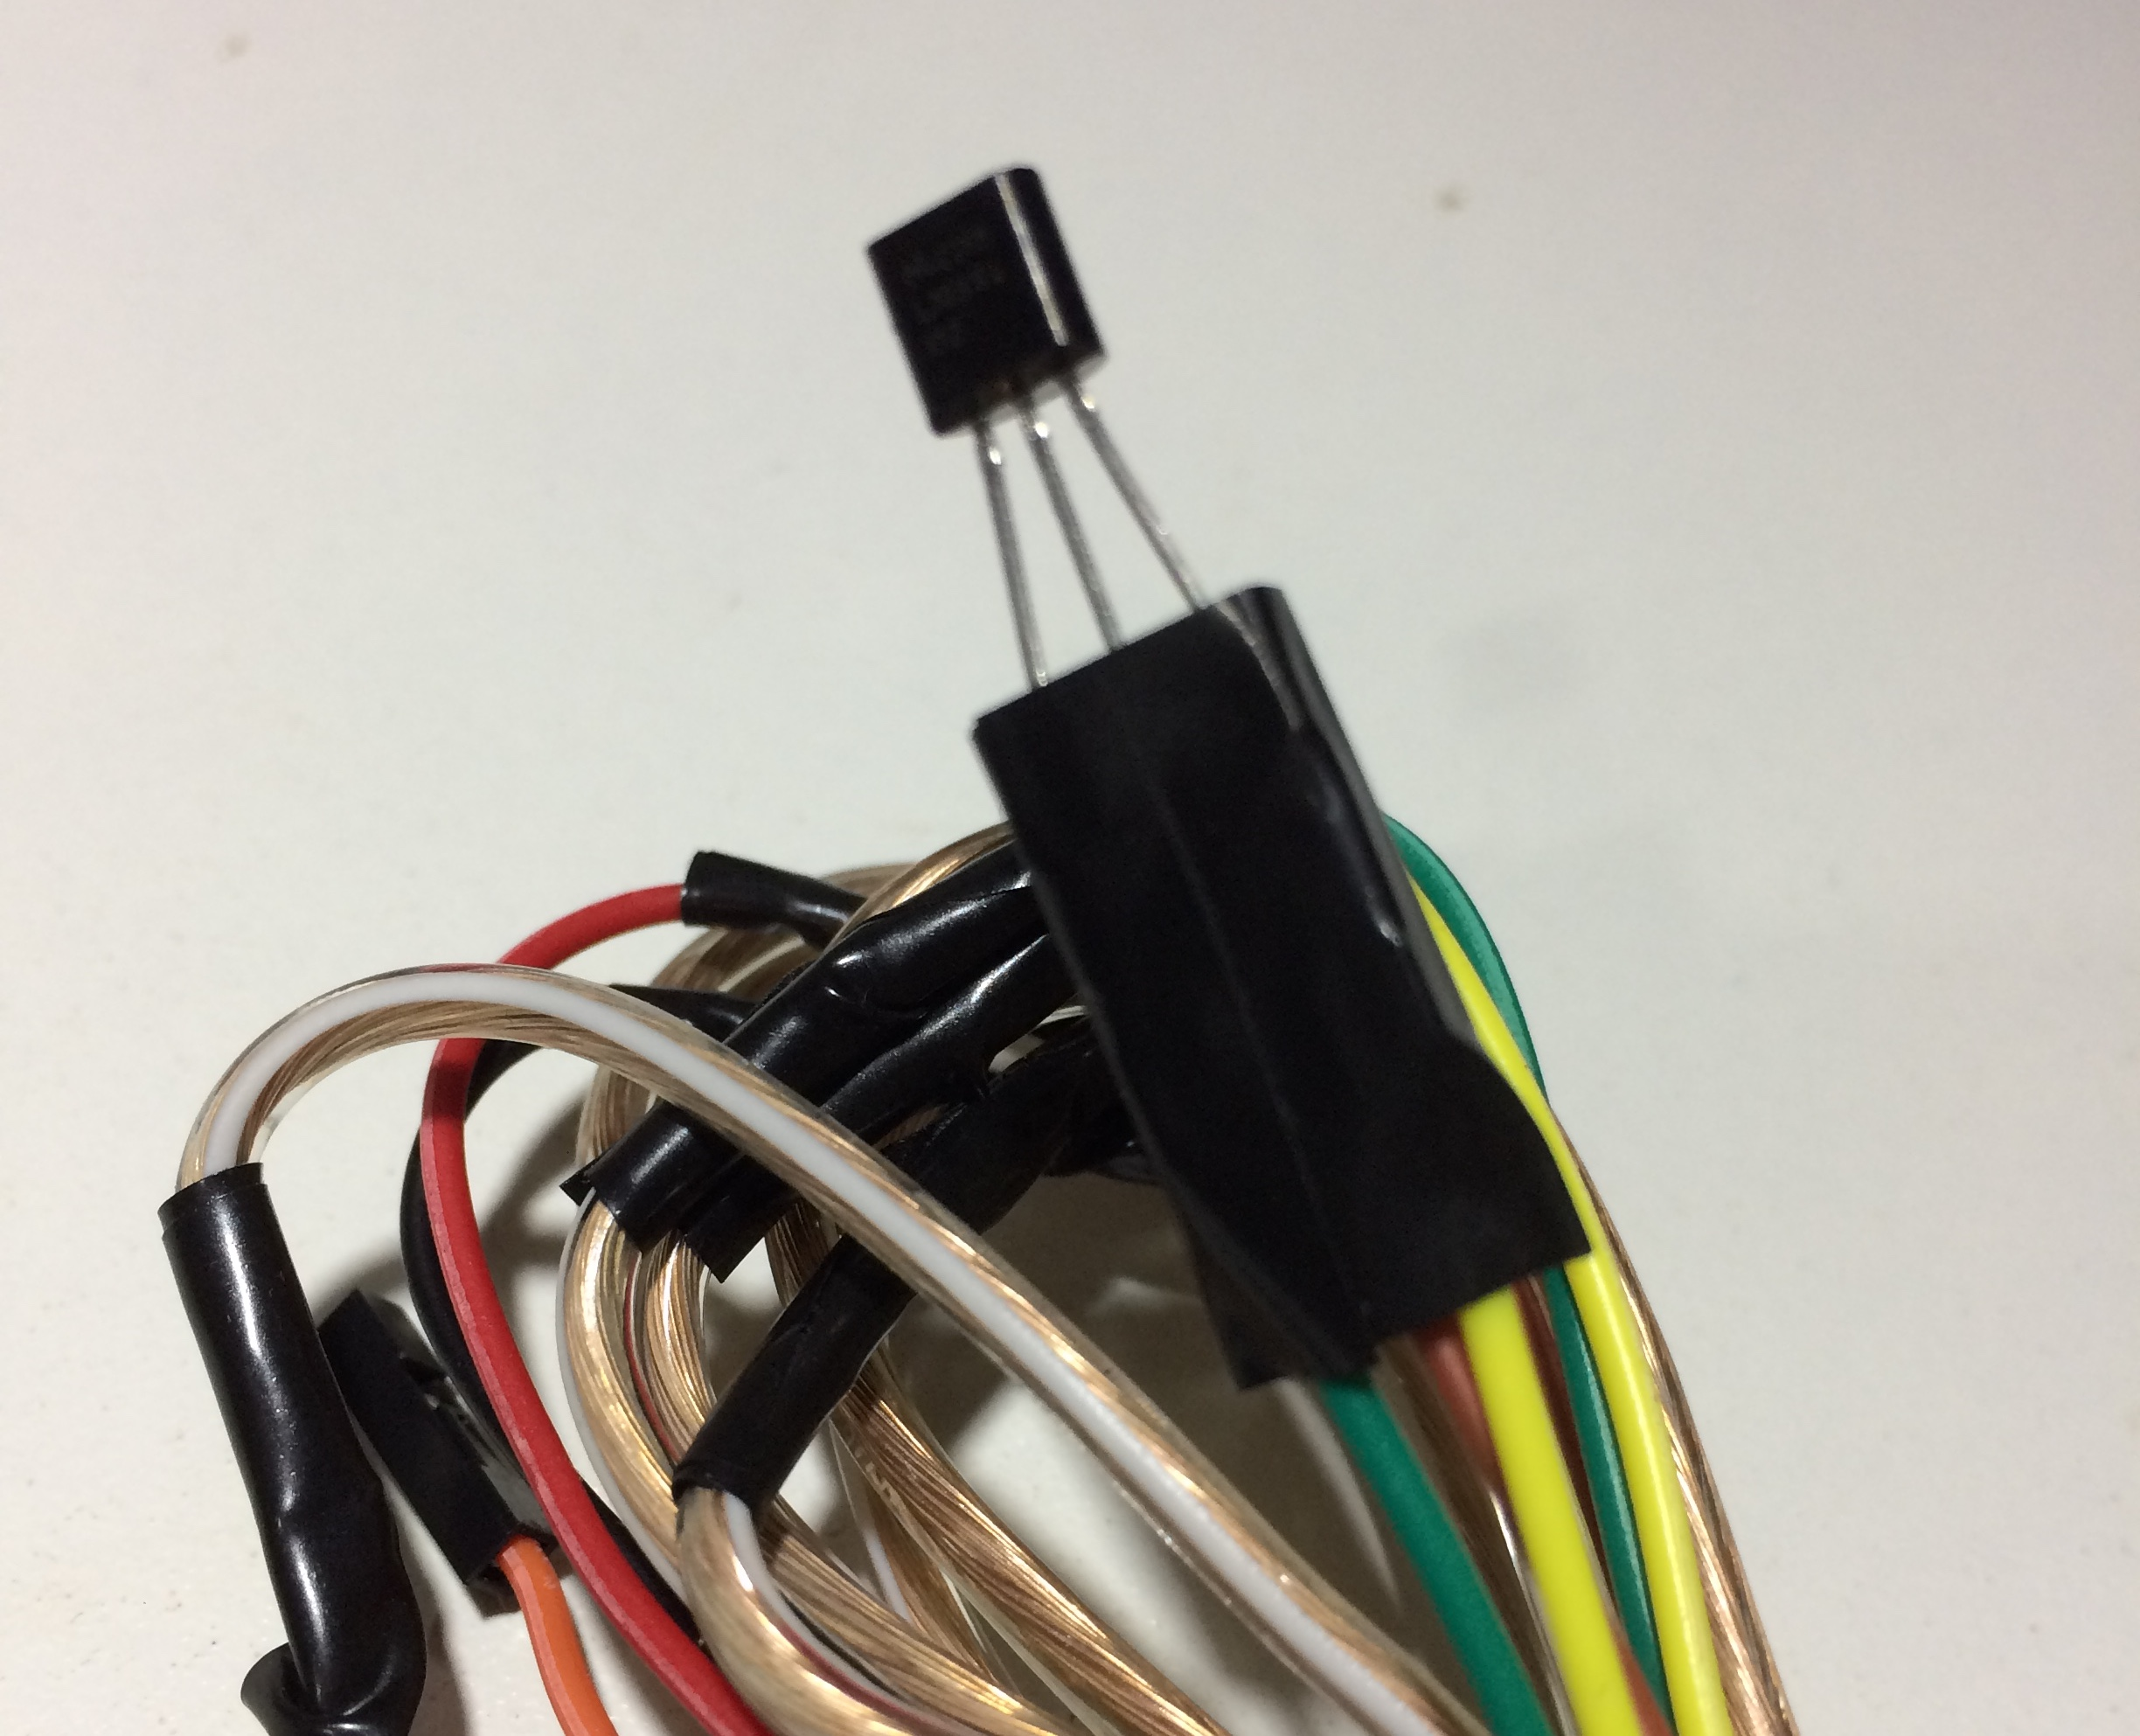
\includegraphics[scale=0.075]{figuras/temp_ele.jpg}
    \end{center}
    \caption{Sensor para medição de temperatura corporal.}
    \label{fig:tempele}
\end{figure}


O sistema de monitoramento de sinais de resistência galvânica da pele (GSR),
tem como principal função o monitoramento de variações na umidade da pele do
usuário, podendo indicar níveis perigosos de estresse ou até mesmo colapsos de
hipoglicemia ou por fraqueza por falta de alimentação. O sistema consiste em
dois eletrodos fabricados, como visto na Figura \ref{fig:gsrele}, para contato com o
antebraço do usuário, com uma distância fixa de 5 $cm$ entre eles, dessa forma,
mantendo os valores das medições confiáveis para cada usuário com diferentes tipos de pele.

\begin{figure}[h!]
    \begin{center}
        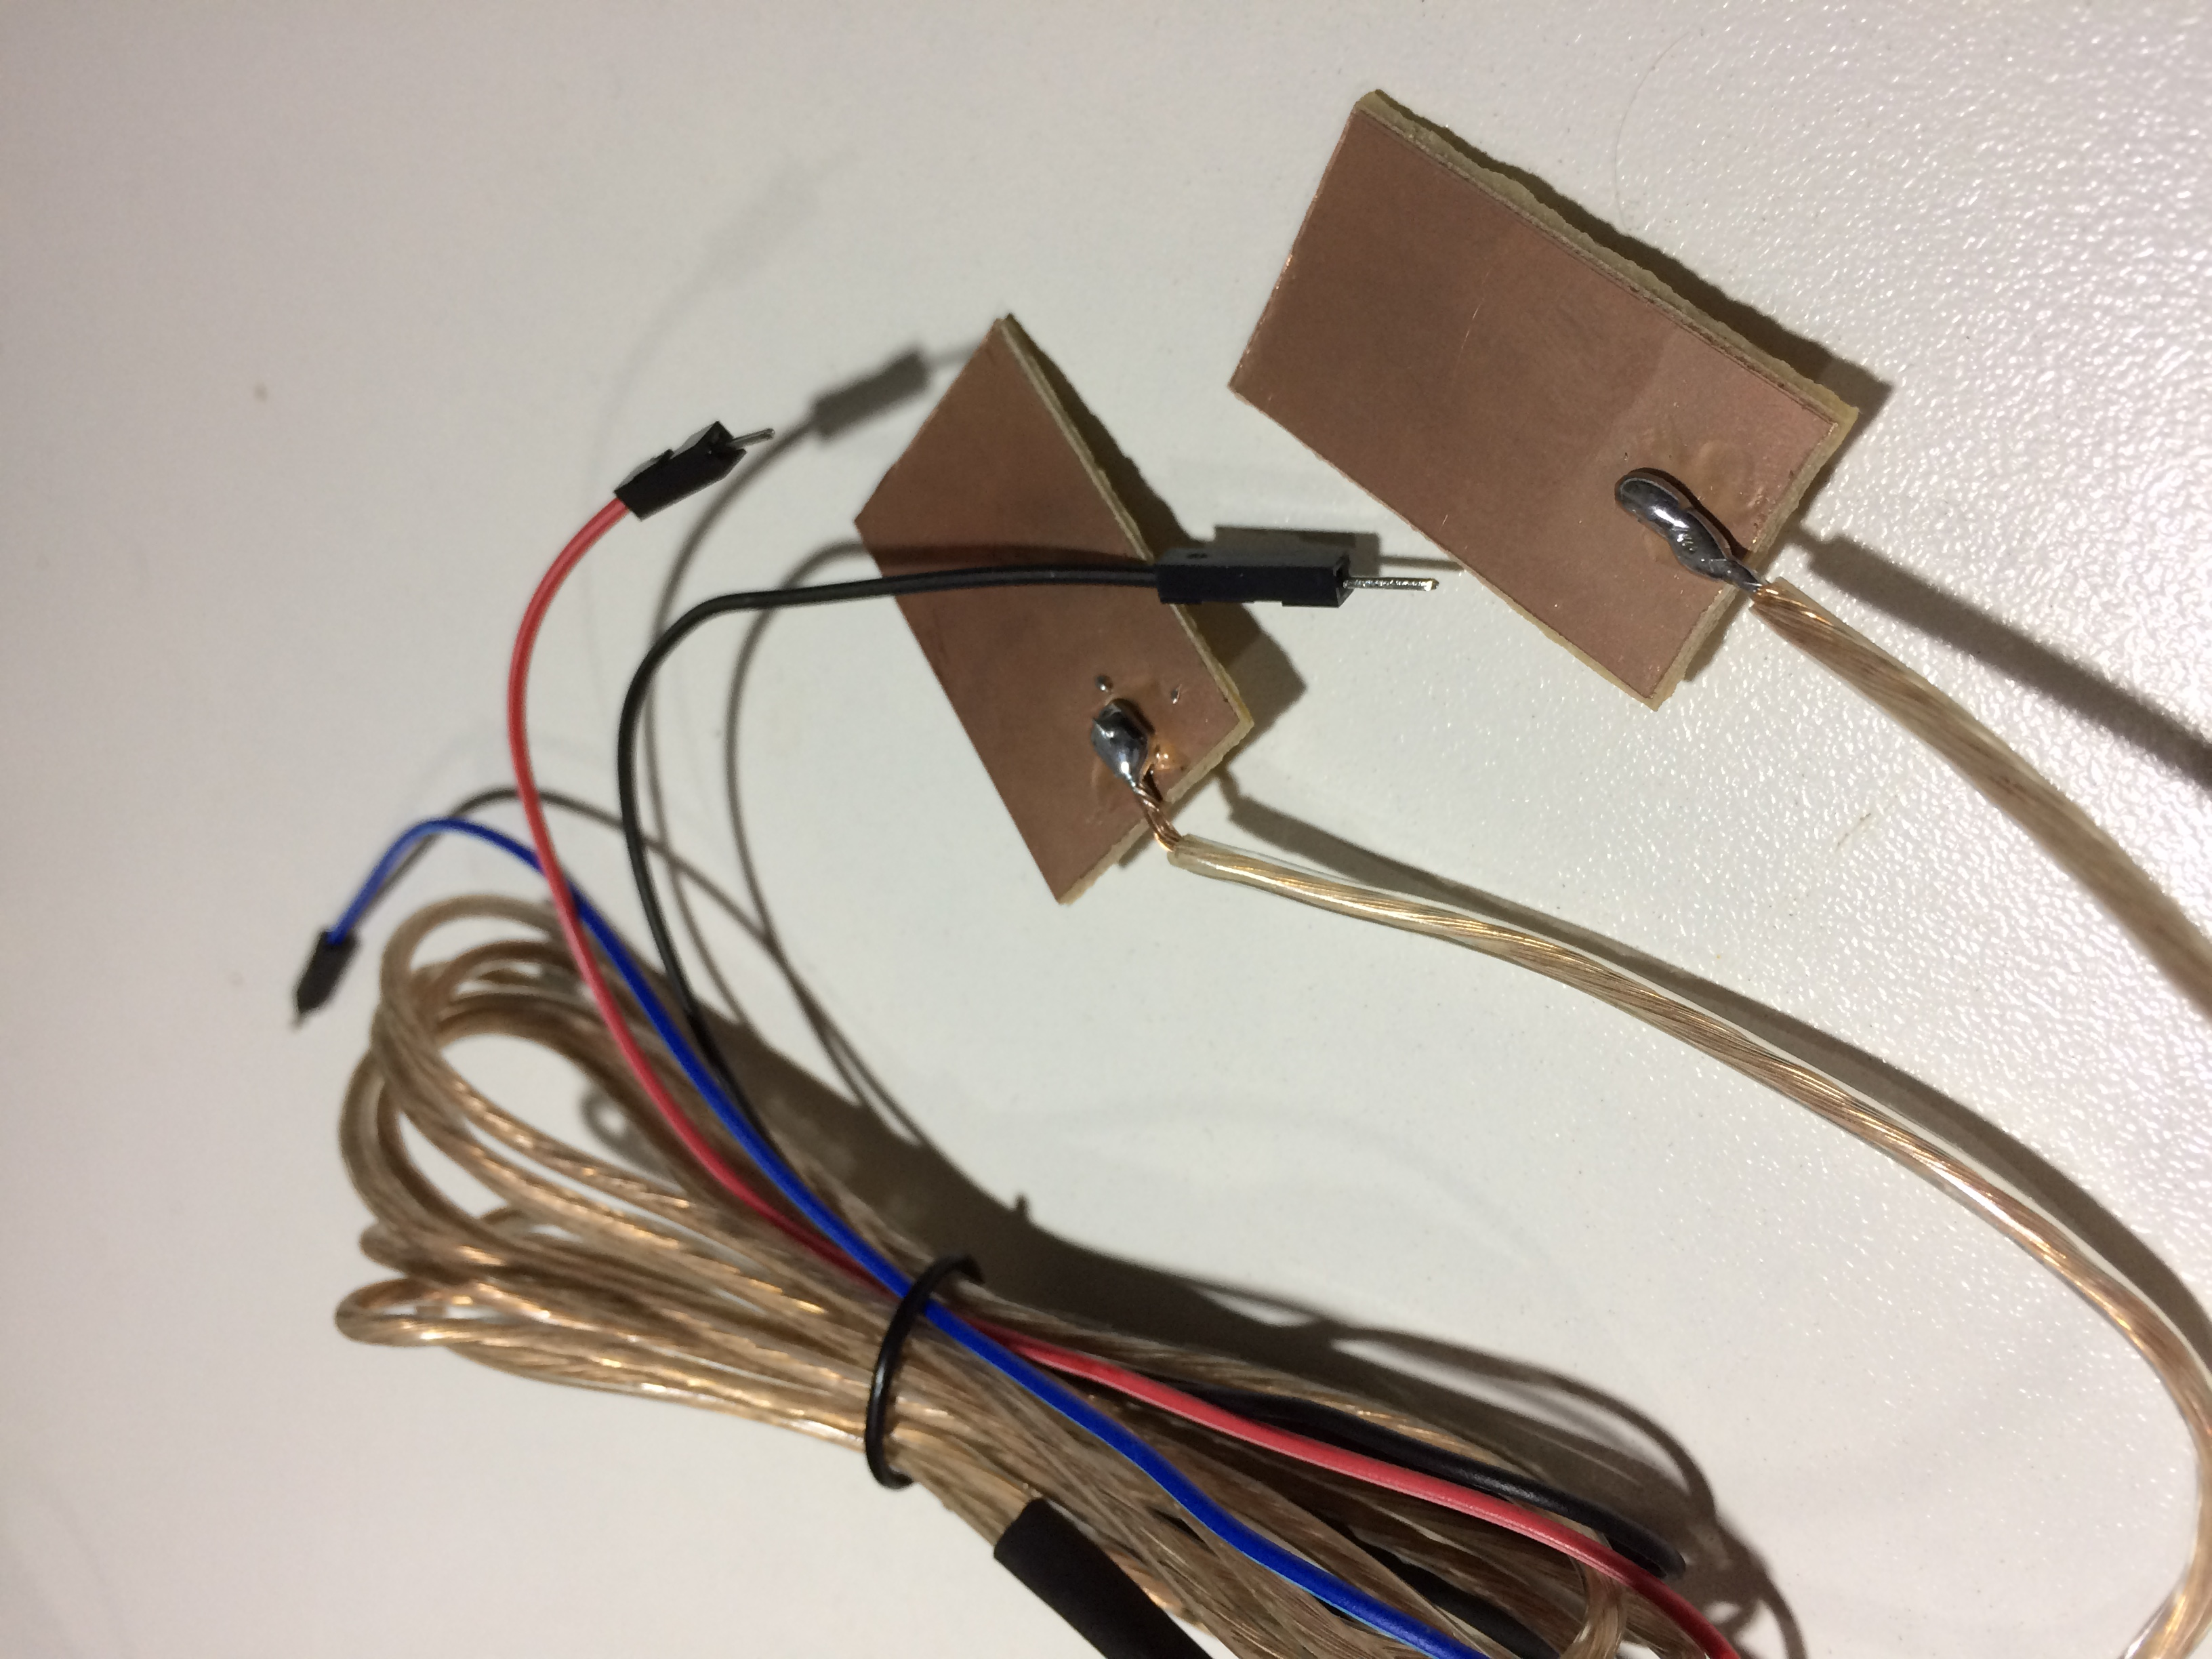
\includegraphics[scale=0.05]{figuras/gsr_ele.jpg}
    \end{center}
    \caption{Eletrodos fabricados para medição de umidade e resistência galvânica da pele.}
    \label{fig:gsrele}
\end{figure}

Além disso, o circuito, visto na Figura \ref{fig:gsr_circ} embarcado conta com um
capacitor de acoplamento para o contato com a pele
humana e um resistor de alta impedância para a medição da variação da resistência da pele
por divisor de tensão. O sistema foi simplificado para que pudesse ser implementado junto
aos cabos dos eletrodos, de forma a utilizar o mínimo de espaço possível na cadeira de rodas.

\begin{figure}[h!]
    \begin{center}
        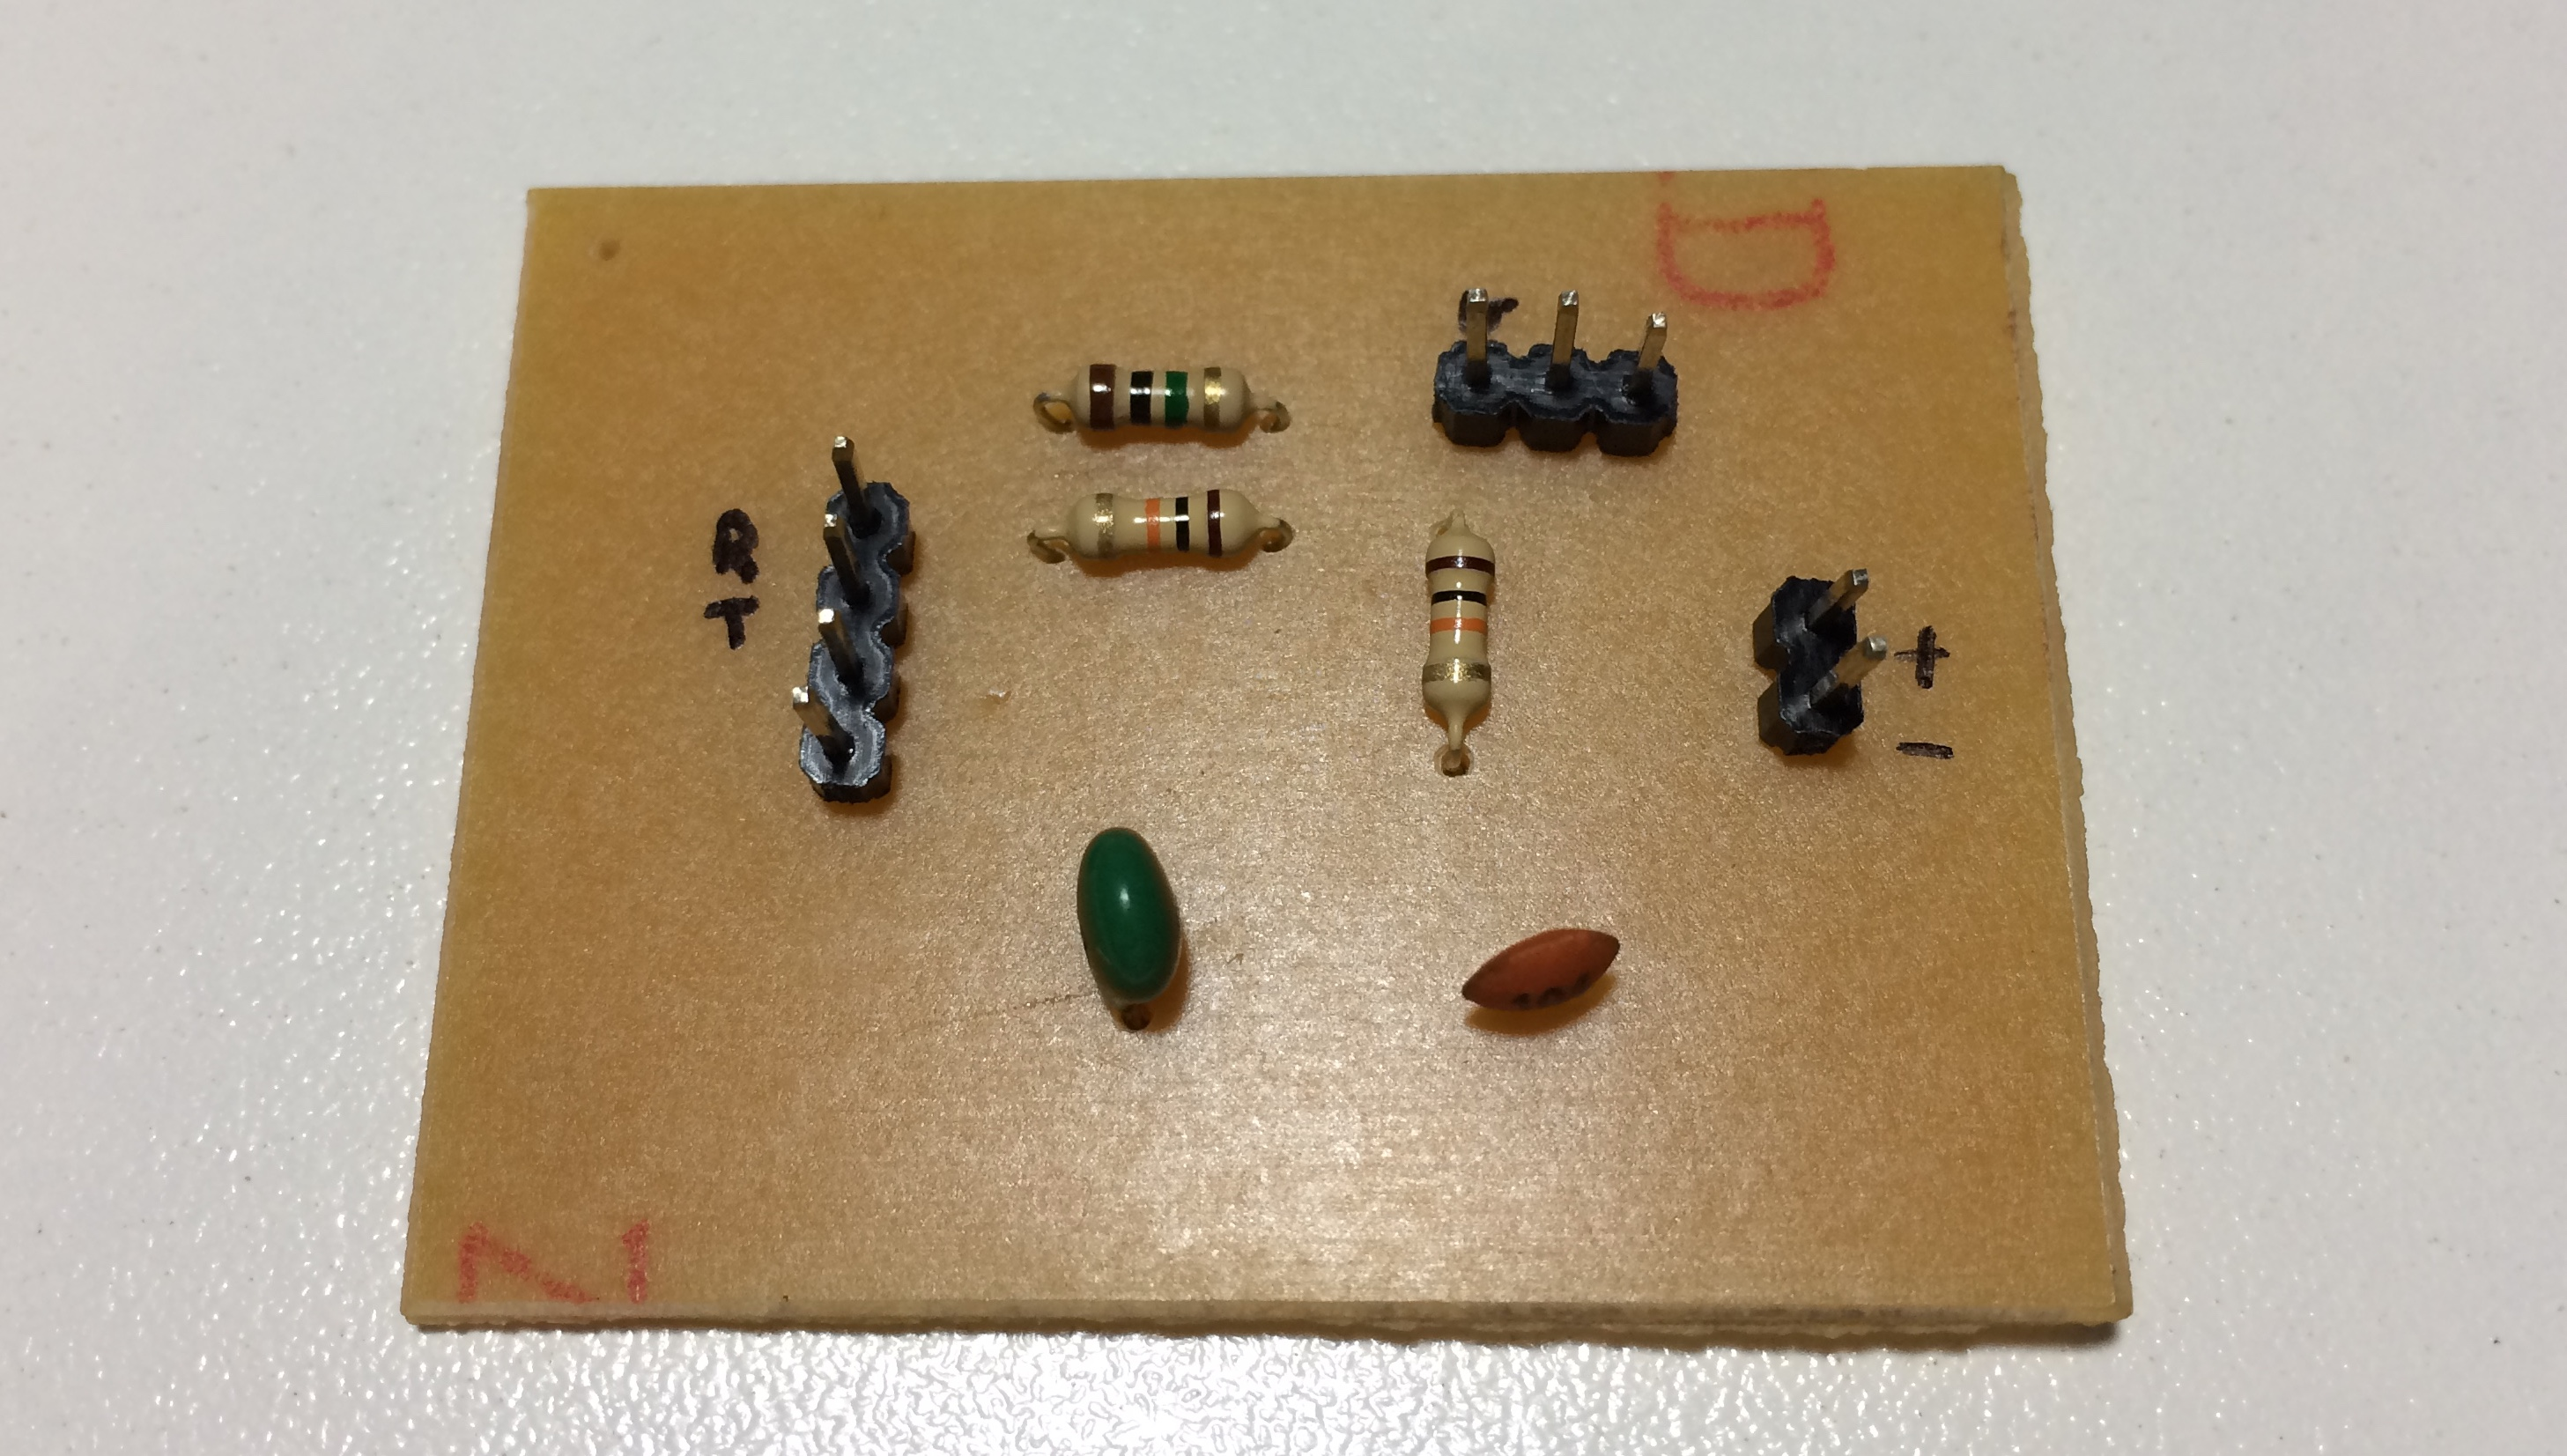
\includegraphics[scale=0.075]{figuras/gsr_circ.jpg}
    \end{center}
    \caption{Circuito para captura de umidade da pele por GSR.}
    \label{fig:gsr_circ}
\end{figure}

O algoritmo para o monitoramento da resistência galvânica e umidade conta com
comparadores para diferentes status do usuário, podendo alertar quando o usuário
não está realizando a medição, quando apresenta características normais para sua
pele ou quando o usuário encontra-se em situação de risco. O sistema embarcado para
o monitoramento e integração com o \textit{middleware} foi programado em linguagem Python.

O sistema de alerta de quedas é responsável por enviar alertas para o servidor
caso o usuário encontre-se fora da cadeira, indicando que o mesmo caiu da cadeira
e necessita de auxílio urgente. Para esse sistema, apresentado na Figura \ref{fig:fall_ele} foi desenvolvido um circuito
com um sistema de medição de distância e presença utilizando um módulo com sensor
piezoelétrico. O sistema é responsável pelo monitoramento de variações de tensão
no sensor, possibilitando o processamento dessa variação, alertando a presença
ou não do usuário na cadeira de rodas. O sensor piezoelétrico é inserido no assento
da cadeira para que o mesmo esteja pressionado durante todo o momento que o usuário
esteja sentado na cadeira, e dessa forma, o algoritmo é capaz de alertar caso a
presença do usuário na cadeira não seja identificada.

\begin{figure}[h!]
    \begin{center}
        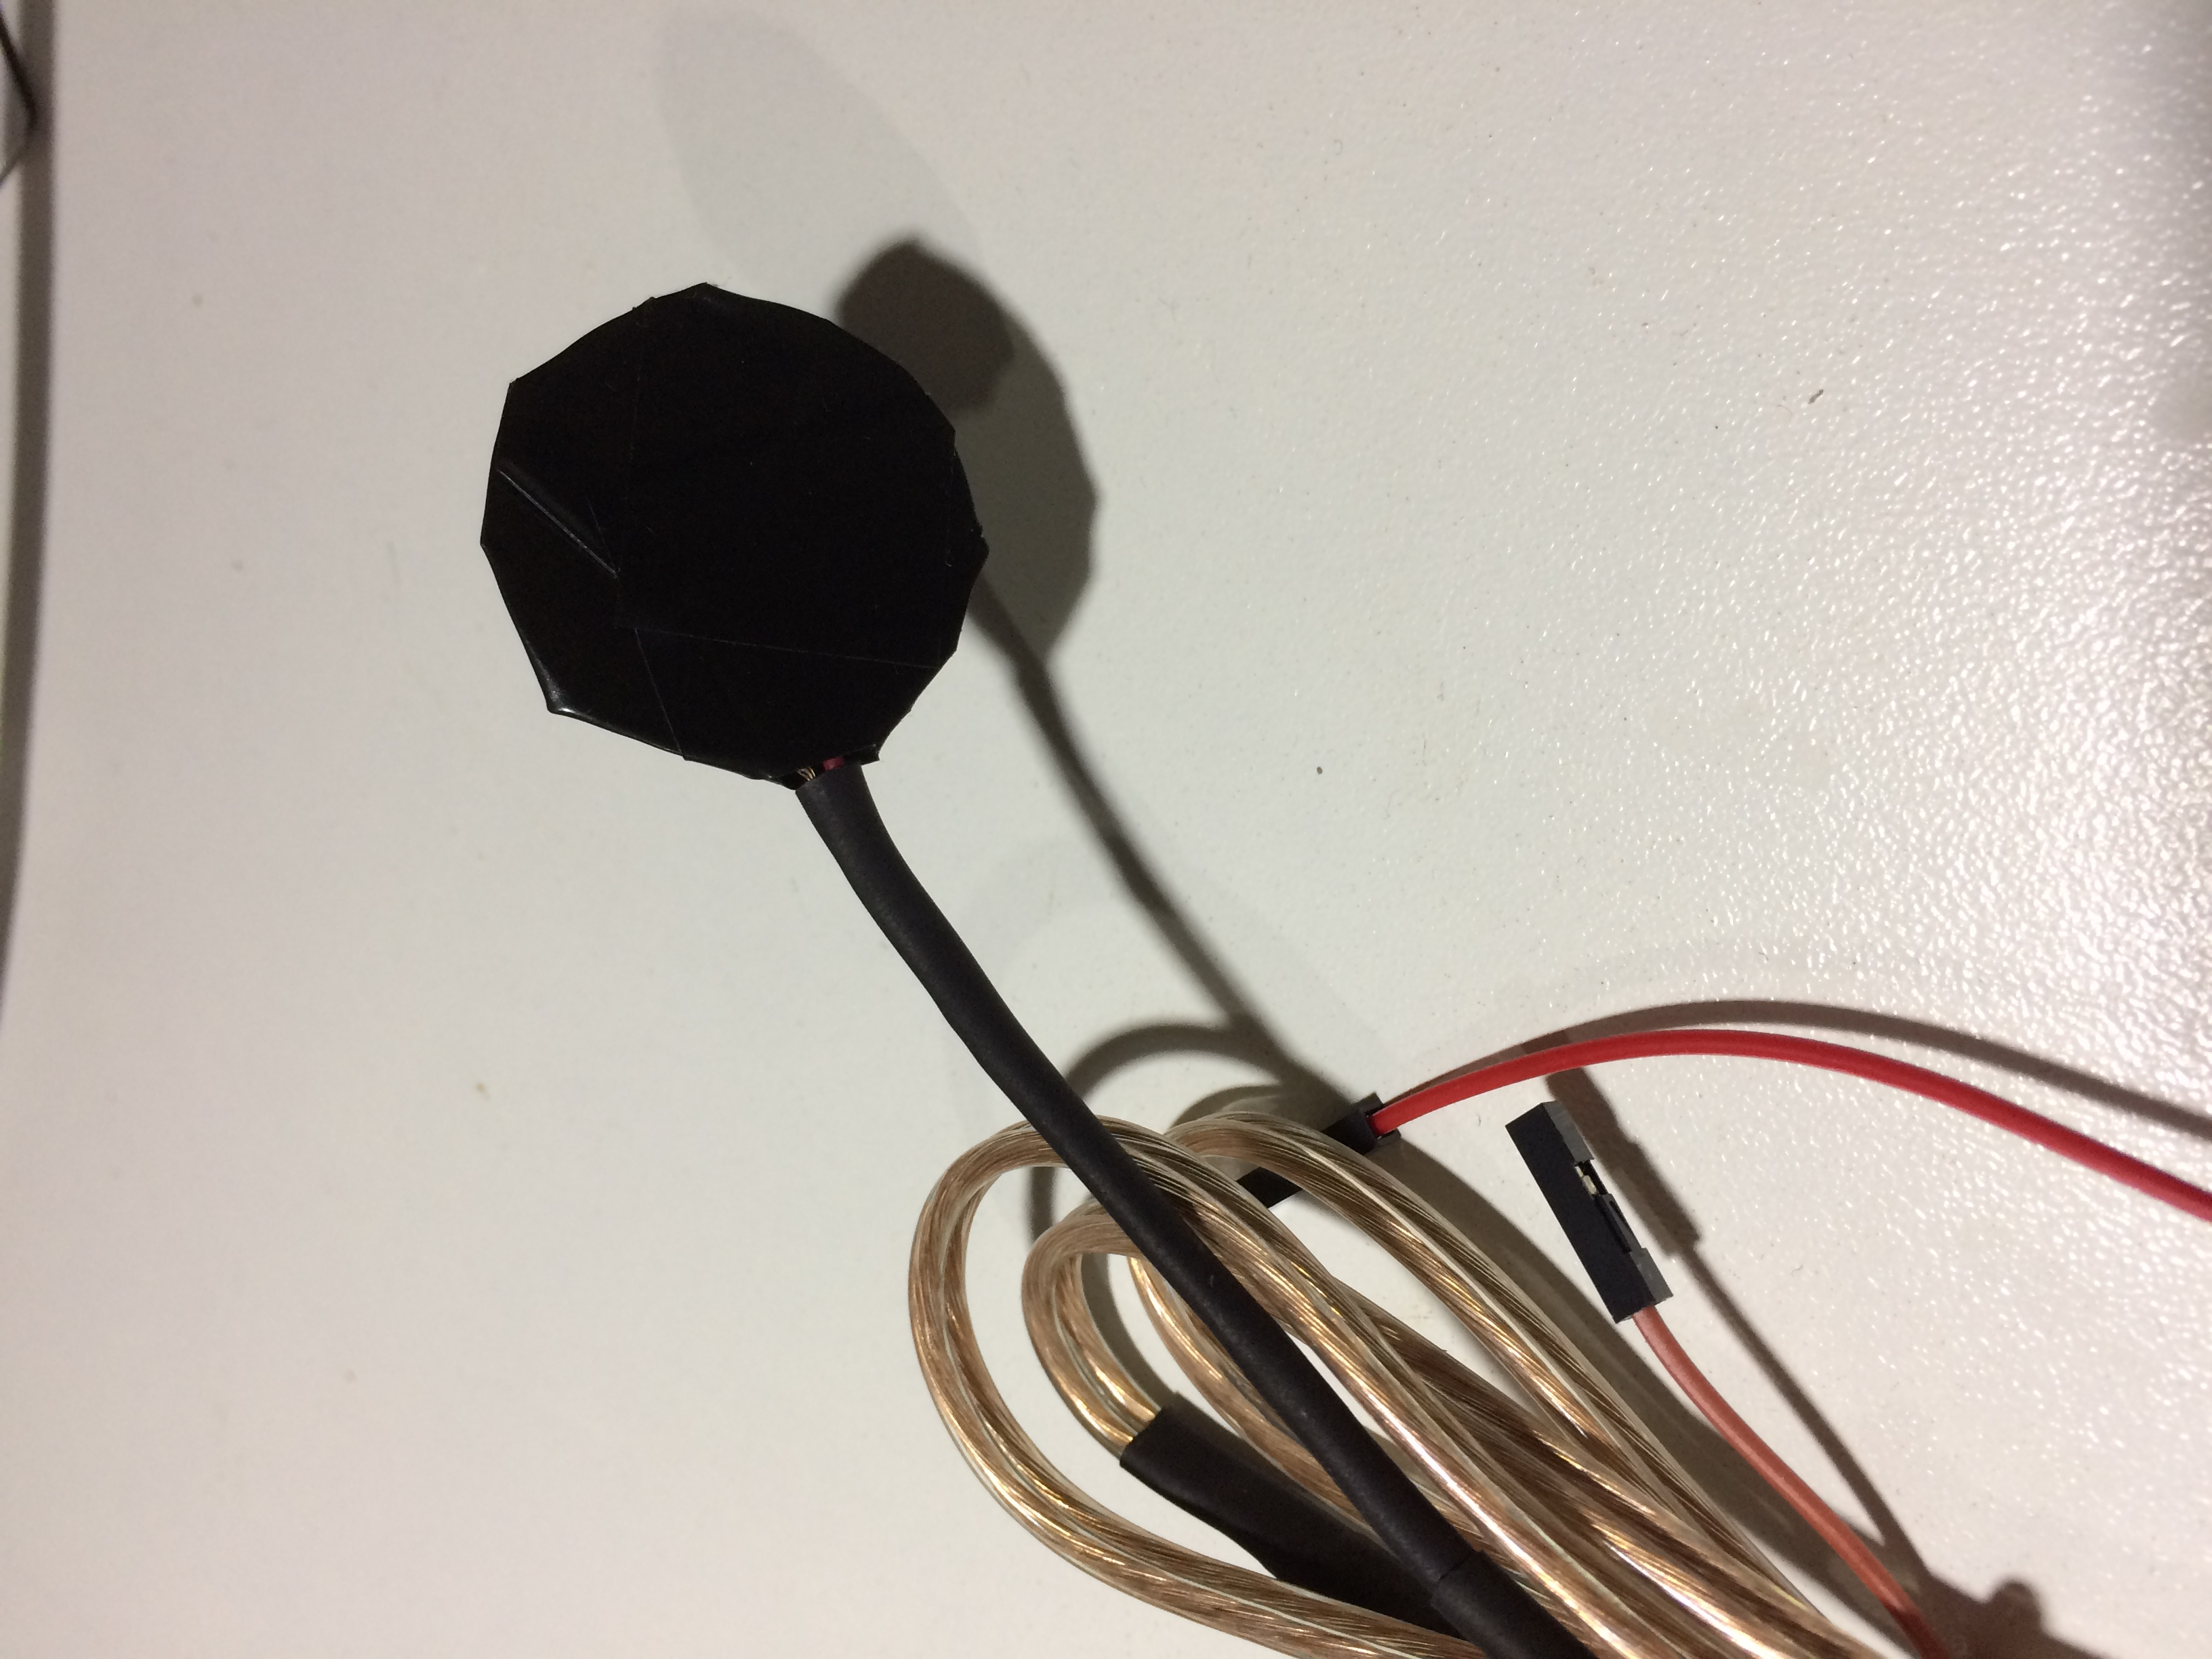
\includegraphics[scale=0.05]{figuras/fall_circ.jpg}
    \end{center}
    \caption{Sensor de presença do usuário na cadeira de rodas.}
    \label{fig:fall_ele}
\end{figure}

O sistema de monitoramento dos sinais de eletrocardiografia 
foi desenvolvido para captura dos sinais de pulso cardíaco com um sensor 
fotoelétrico e um LED verde de alto brilho, a partir de sinais de PPG (photoplethysmografia), 
para que as medidas e a captura do sinais seja
feita da forma menos invasiva possível. Para isso, o circuito deve ser capaz de
capturar o sinal de pulso cardíaco por meio ótico com precisão e assim, foi 
utilizado o sensor SEN-11574, apresentado na Figura \ref{fig:ecg_circ}, 
baseado em um amplificador operacional MCP6001, 
que possui produto ganho-banda de 1MHz e possui aplicações específicas para 
amplificação de sinais provenientes de fotodiodos e fototransistores. Além disso, 
o sistema consiste em um LED de alto brilho de cor verde e um sensor fotodiodo 
APDS9008 de alta sensibilidade a variações de iluminação, capaz de capturar sinais 
de PPG com a passagem e retorno de luz pelo tecido humano.
Além do amplificador e do sensor selecionado, foram projetados filtros passa-alta para
rejeição de frequências abaixo de 0.7Hz que possam aplicar um nível DC no sinal,
que acabam tendo papel fundamental na etapa de captura da frequência cardíaca 
pois elevam o sinal, dificultando a captura da frequência por meio de um algoritmo 
presente no sistema de processamento digital. O circuito utilizado é dado pelo 
esquemático apresentado na Figura \ref{fig:ecg_sch}

\begin{figure}[h!]
    \begin{center}
        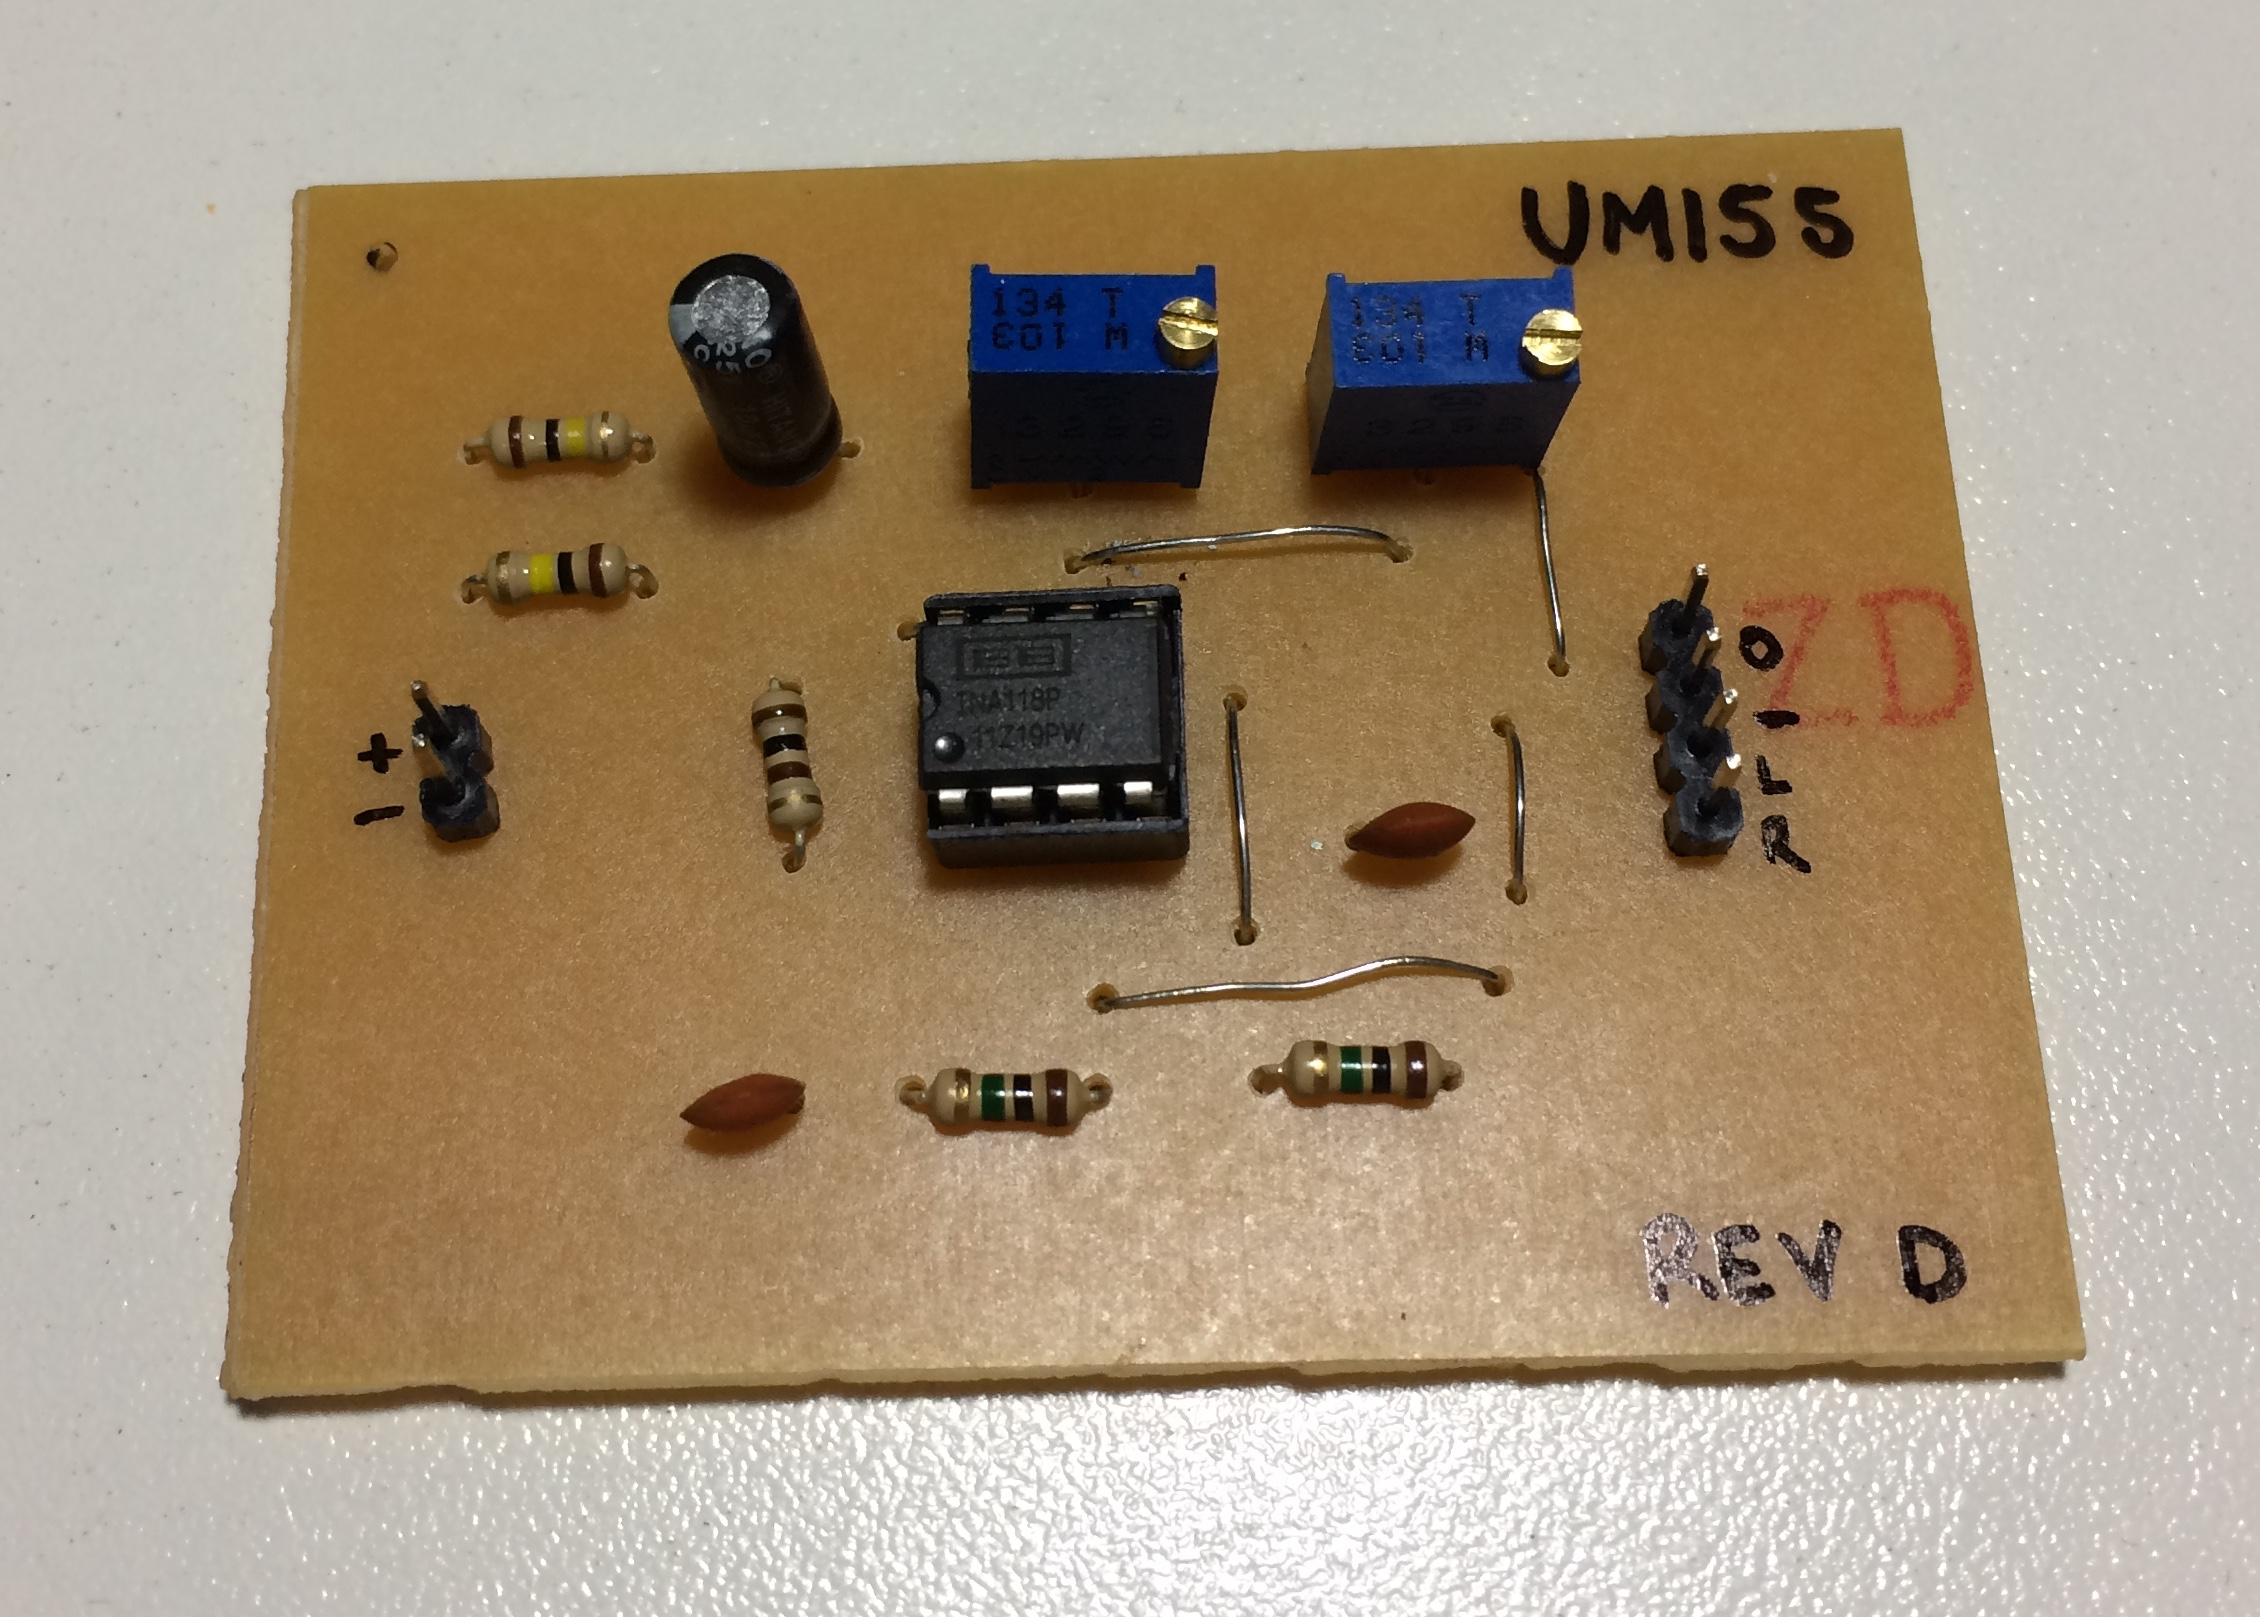
\includegraphics[scale=0.4]{figuras/ecg_circ.jpg}
    \end{center}
    \caption{Sensor ótico para captura de sinais PPG da fabricante \textit{SparksFun}}
    \label{fig:ecg_circ}
\end{figure}

\begin{figure}[h!]
    \begin{center}
        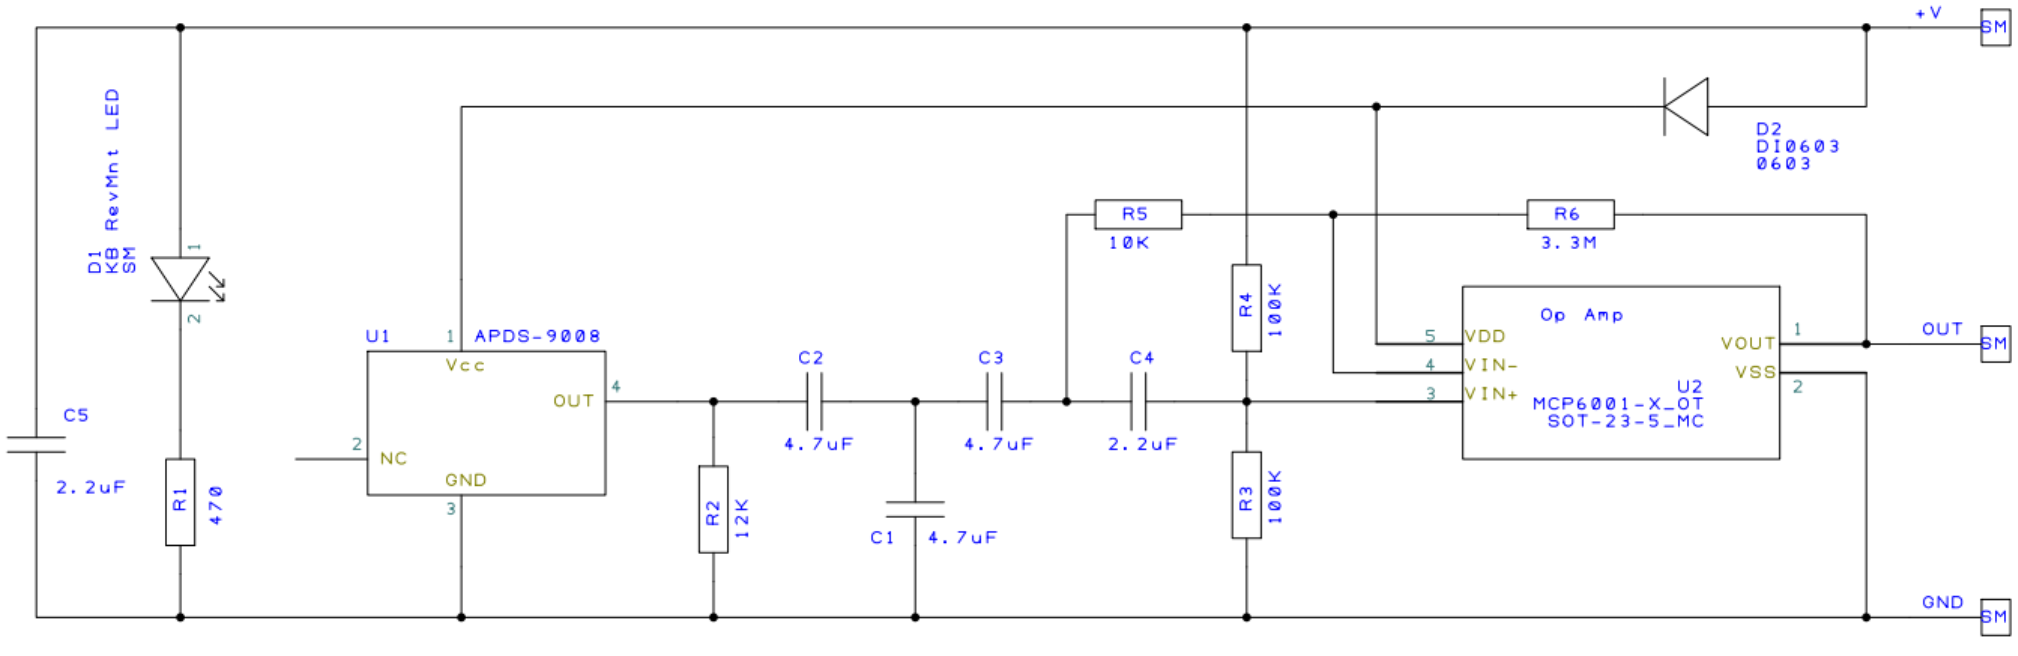
\includegraphics[scale=0.4]{figuras/ecg_sch.png}
    \end{center}
    \caption{Esquemático do circuito condicionador de sinais PPG proposto pela fabricante}
    \label{fig:ecg_sch}
\end{figure}

É importante ressaltar que os sinais de pulso cardíaco e eletrocardiograma variam 
entre as baixas frequências de 0.5Hz e 40Hz\footnote{ Yazıcıoglu RF, van Hoof C,
Puers R. Biopotential Readout Circuits for Portable Acquisition Systems, 2009,
Springer Science, ISBN: 978-1-4020-9092-9)}, e dessa forma os sistemas de 
condicionamento foram projetados de forma a atenuar frequências maiores que 40Hz 
enquanto aplicam um alto ganho de tensão AC para a leitura do sinal original de 
baixa amplitude, entre 0.1 mV e 5 mV. O módulo do ganho de tensão AC do sinal é dado pelo ganho do 
amplificador MCP6001 em modo não inversor, dado por:

\begin{equation}
  Av = 1 + \frac{3.3M}{10k} = 330
\end{equation}

Com esse ganho, é possível obter os valores de pico dos pulsos cadíacos na faixa 
de 1.65 V.

O algoritmo de captura da frequência cardíaca via sinais de PPG foi desenvolvido 
a fim de calcular o período entre sinais de pulsos sistólicos, eliminando a 
ocorrência de pulsos diastólicos de menor amplitude.

Após a captura e condicionamento de todos os sinais analógicos, os mesmos são direcionados
para um módulo de conversão Analógico-Digital (A/D). O conversor selecionado foi o ADS1115 \footnote{\url{https://cdn-shop.adafruit.com/datasheets/ads1115.pdf}},
devido a sua alta resolução de 16 bits, capaz de converter valores analógicos em valores
digitais de 0 a 65535, e por sua taxa de amostragem de 800Hz, suficientes para a captura dos
sinais a serem monitorados para o projeto. O conversor é conectado com a Raspberry Pi via protocolo I2C,
possibilitando o uso de menos portas para o envio de até 4 sinais simultâneos.

Uma vez com os sinais devidamente convertidos para digital, o sistema embarcado e de \textit{middleware}
é responsável por monitorar os sinais, realizando verificações de seus valores a partir de calibrações
realizadas para cada um dos módulos.

Nas Figuras \ref{fig:psem1} e \ref{fig:psem2} é possível vizualizar o subsistema 
de Processamento de Sinais e Monitoramento integrado à cadeira de rodas do 
projeto.

\begin{figure}[h!]
    \begin{center}
        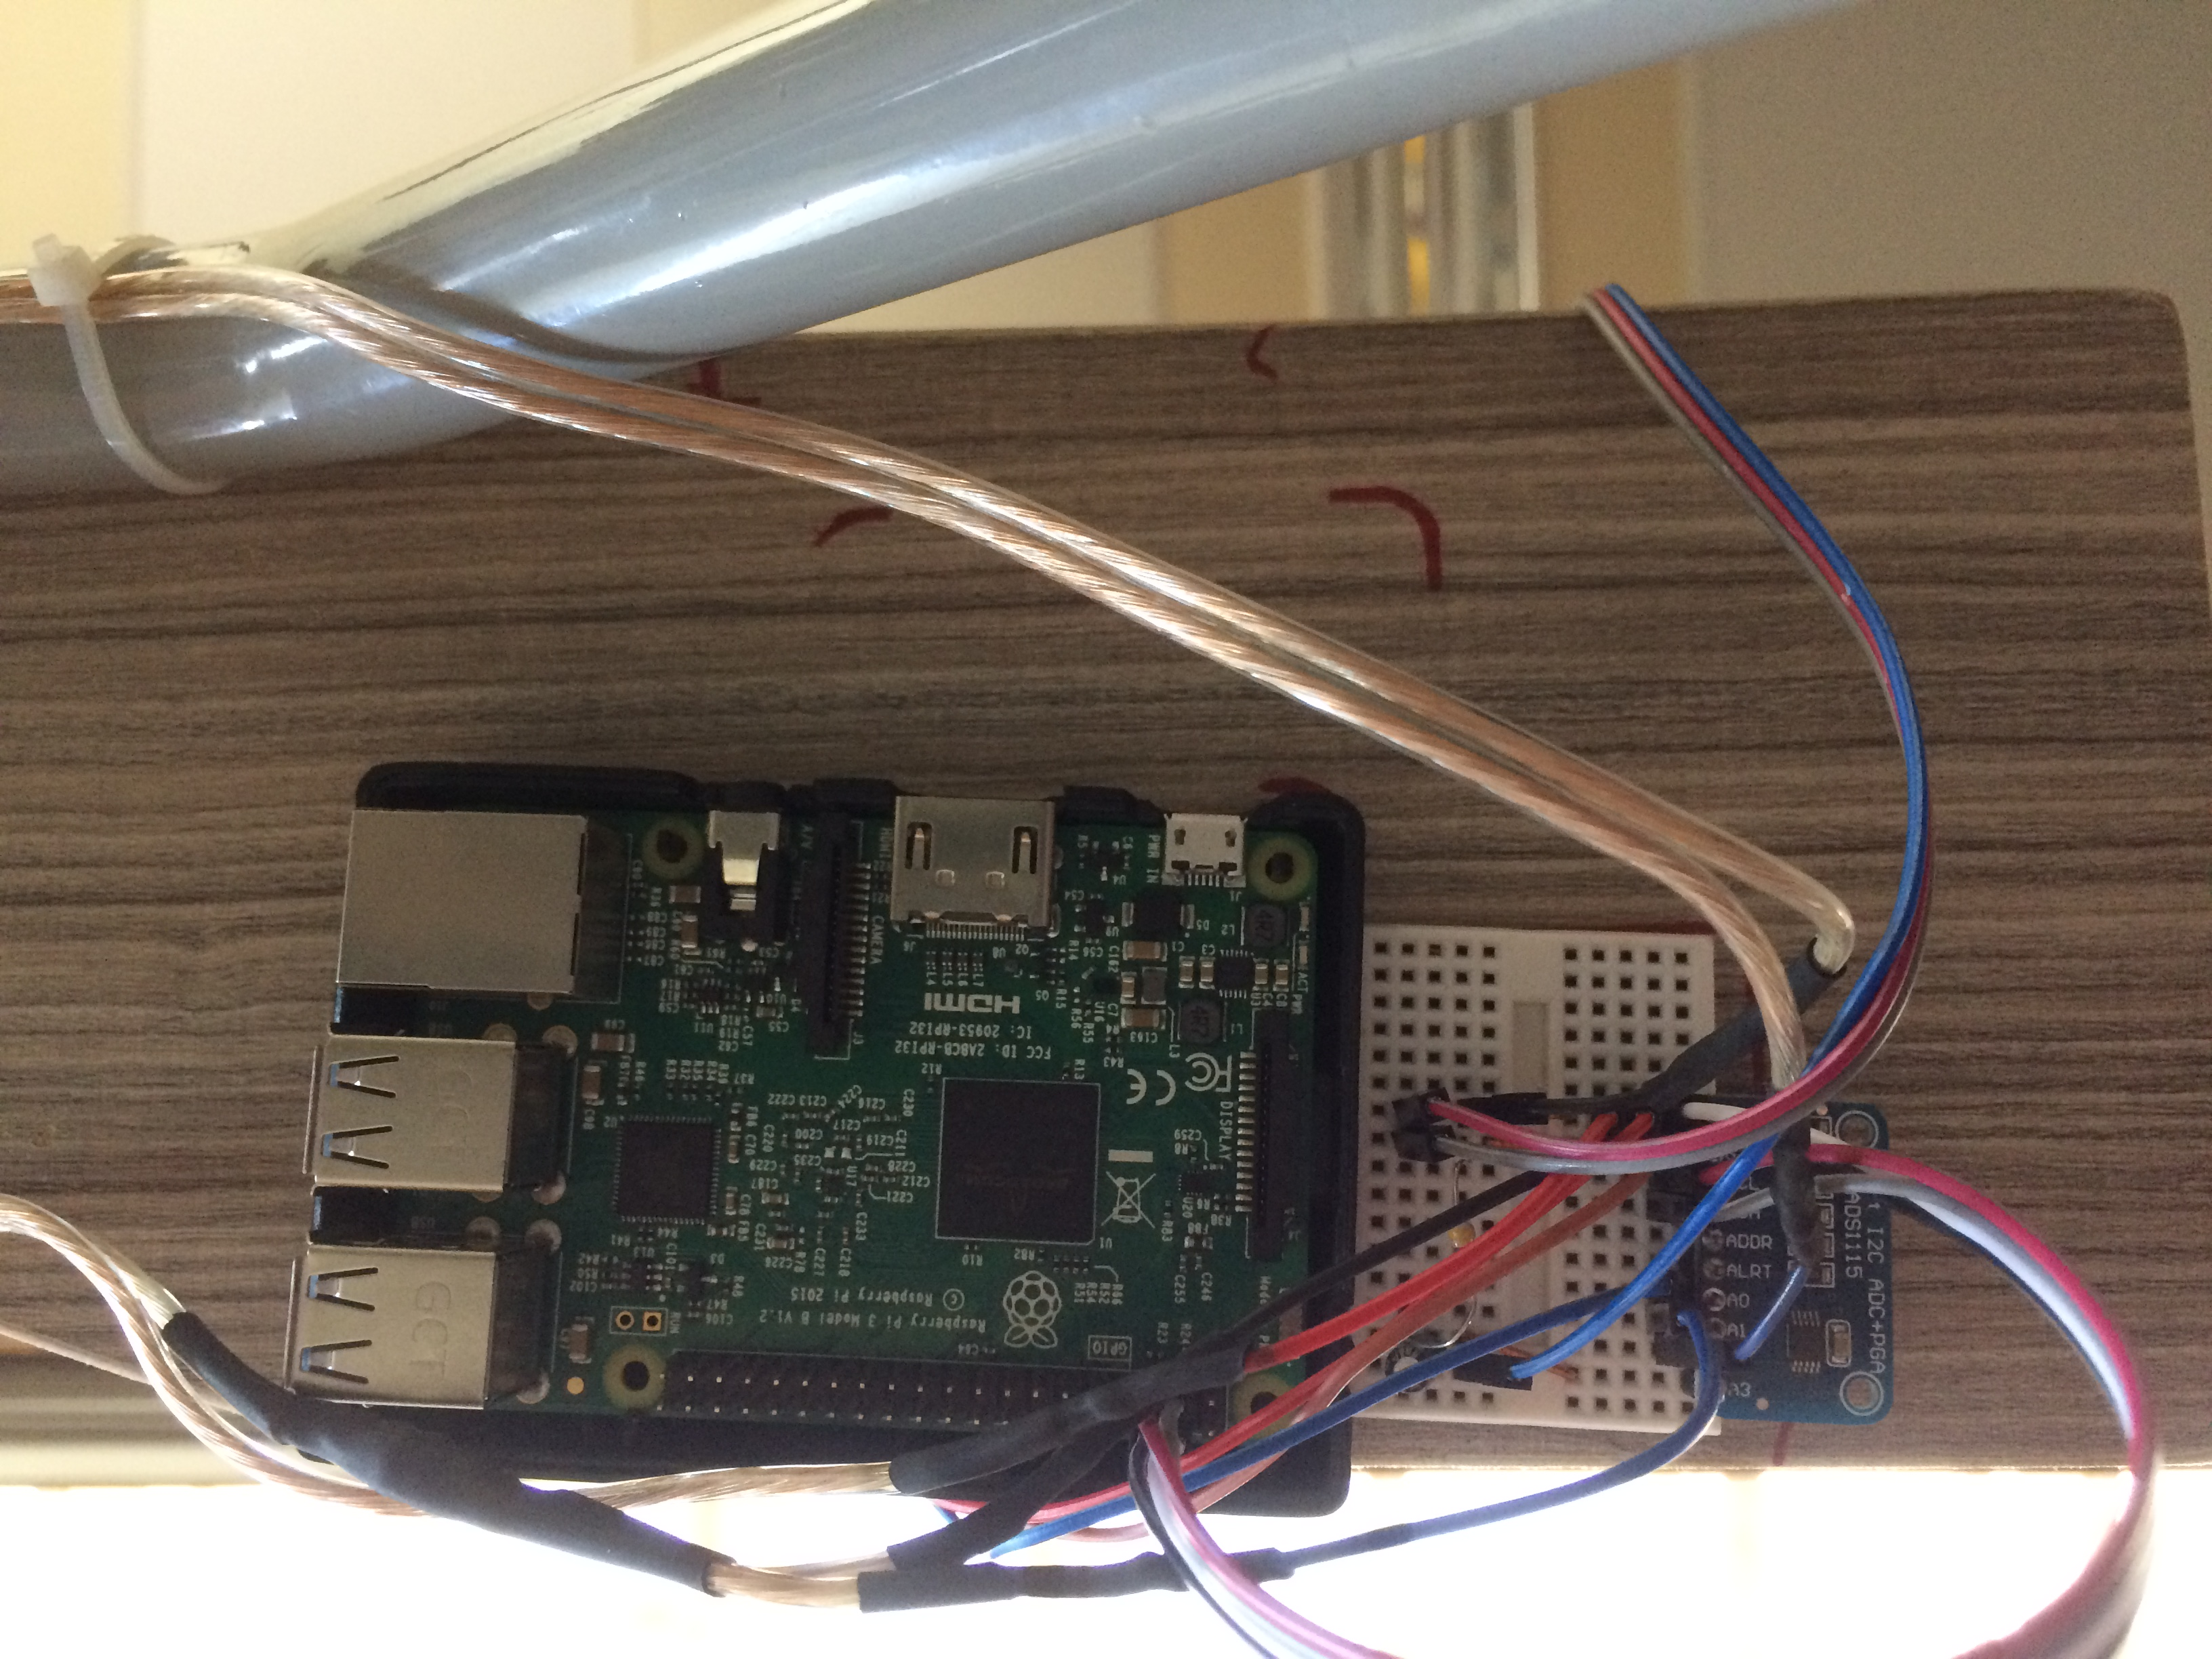
\includegraphics[scale=0.07]{figuras/psem1.jpg}
    \end{center}
    \caption{Esquemático do circuito condicionador de sinais PPG proposto pela fabricante}
    \label{fig:psem1}
\end{figure}

\begin{figure}[h!]
    \begin{center}
        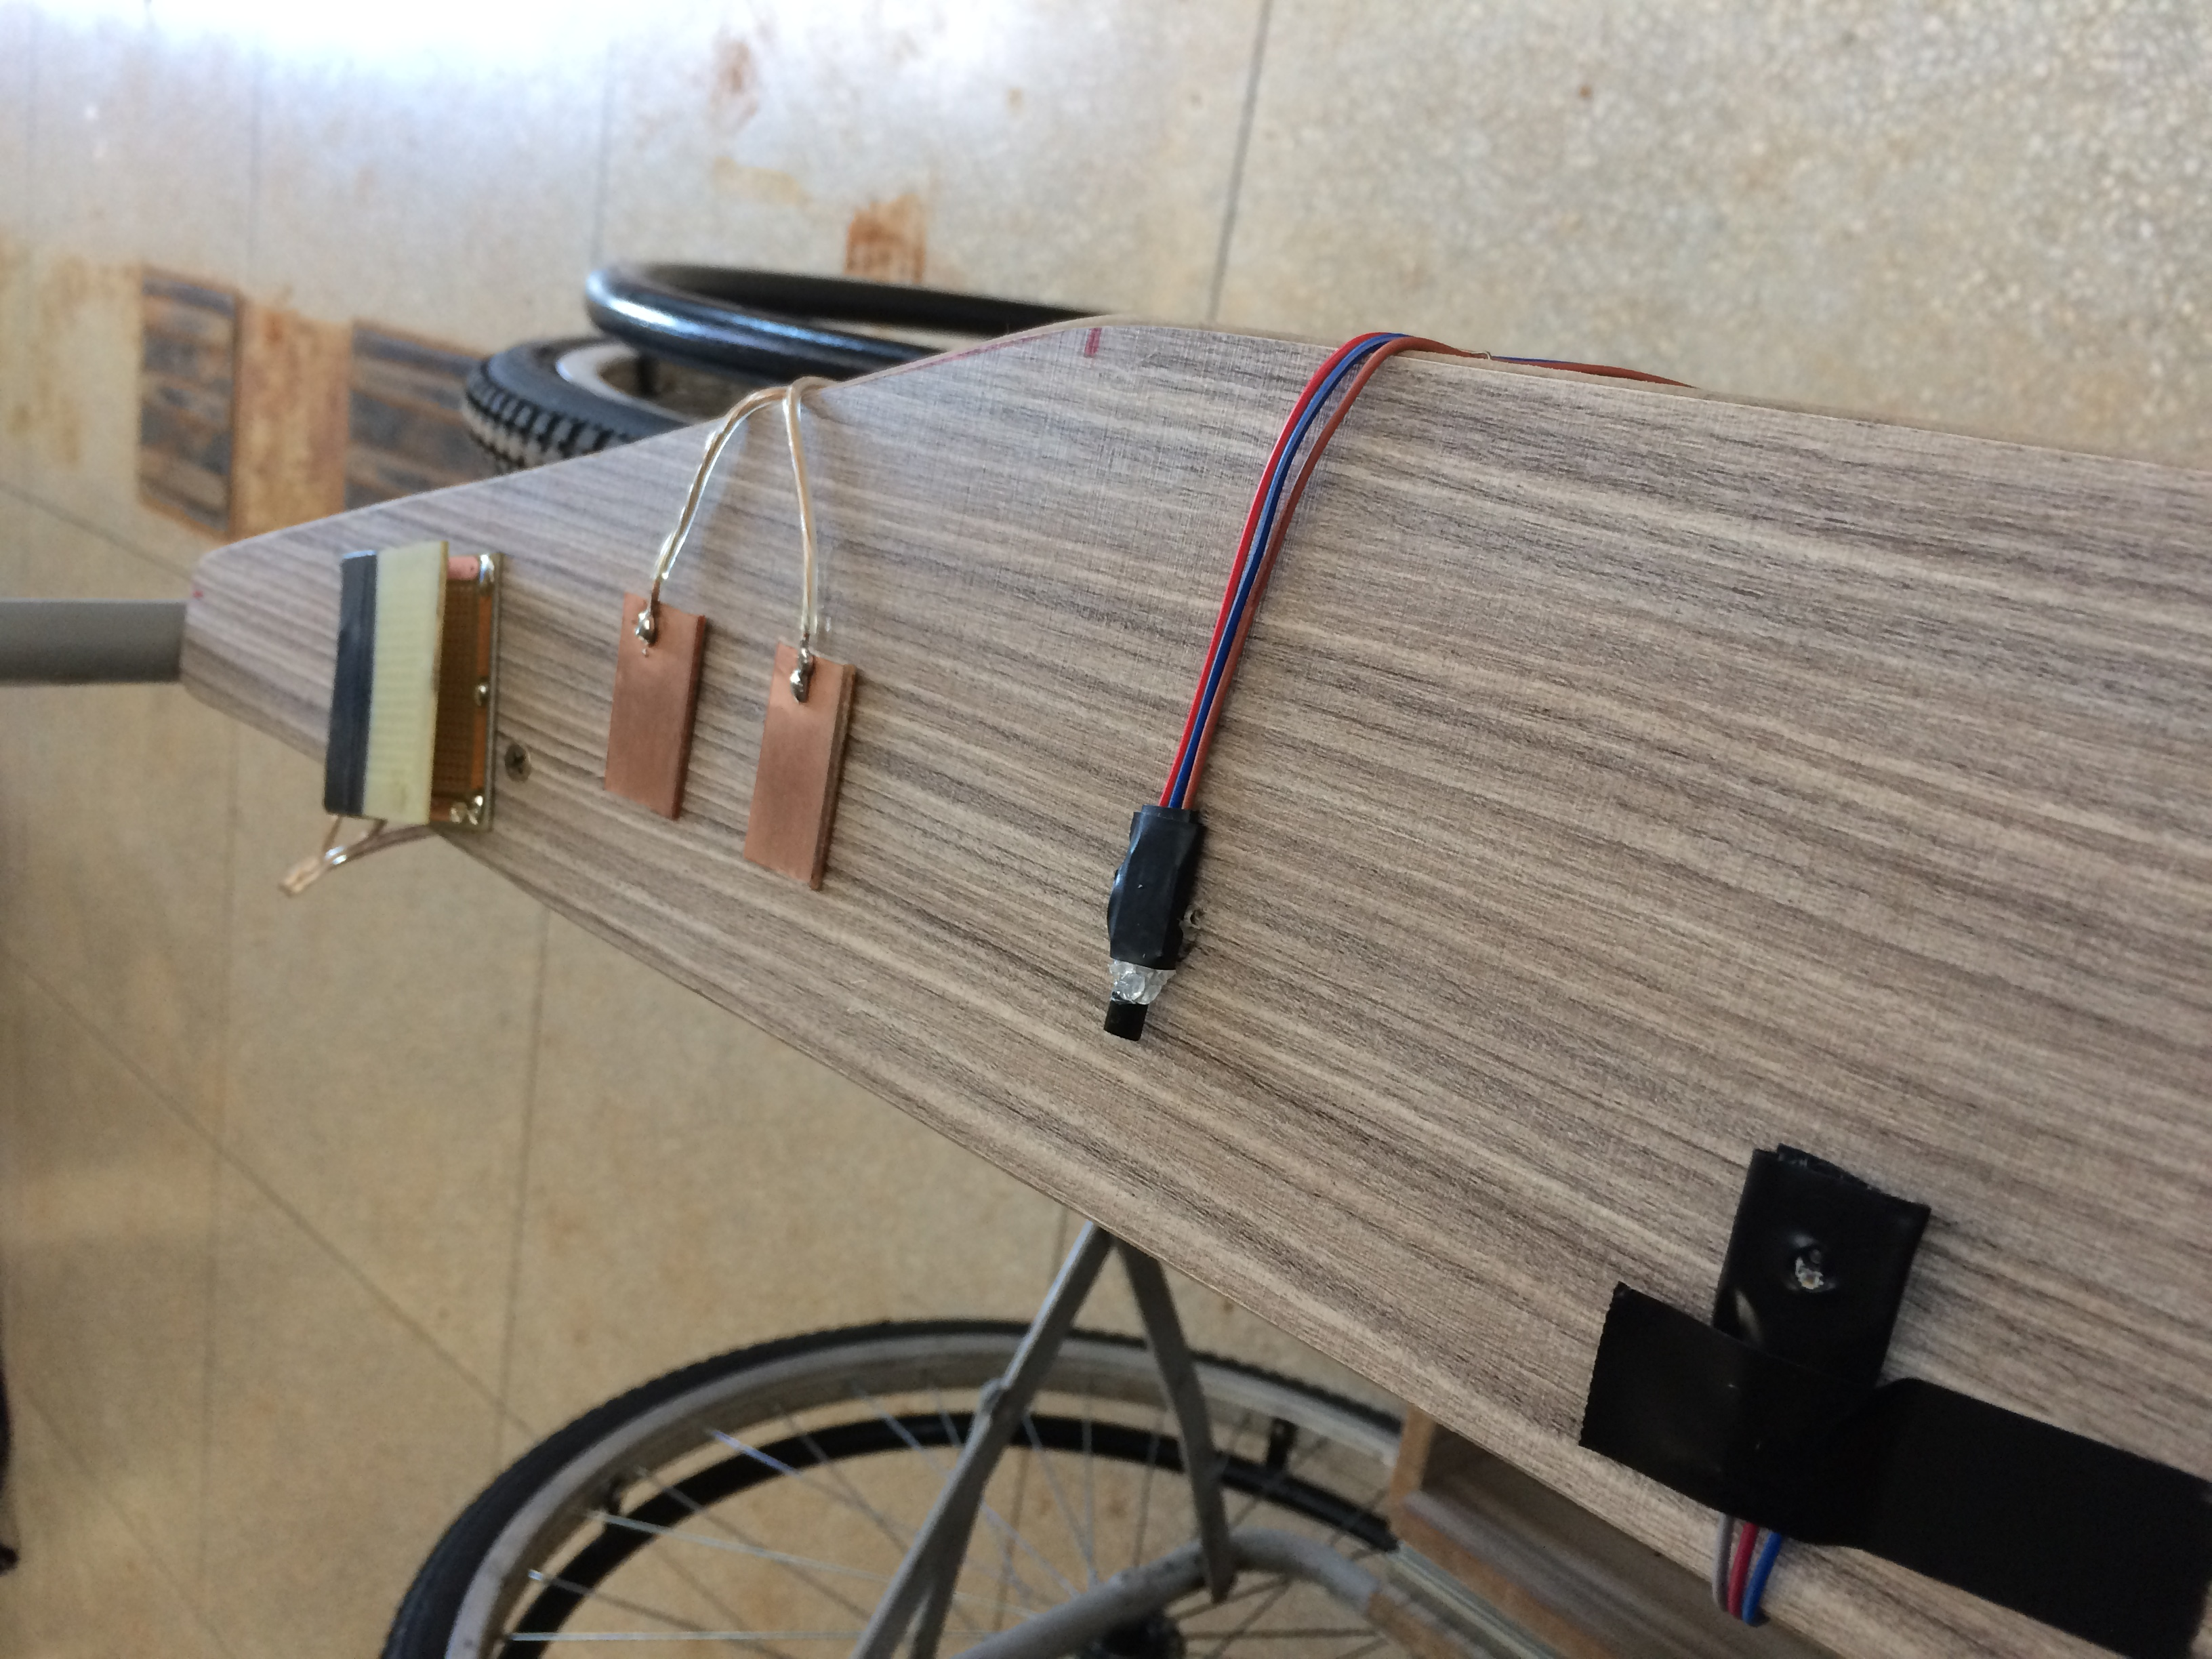
\includegraphics[scale=0.07]{figuras/psem2.jpg}
    \end{center}
    \caption{Esquemático do circuito condicionador de sinais PPG proposto pela fabricante}
    \label{fig:psem2}
\end{figure}
